\documentclass{article}
\usepackage[utf8]{inputenc}
\usepackage[spanish]{babel}
\usepackage{graphicx}
\usepackage{float}

\title{Práctica 4. Primera Parte: Implementación de los ejemplos}
\author{Noelia Escalera Mejías}

\begin{document}
	\maketitle
	\section{Ejemplo 1}
	Se trata de un hello world.
	\begin{itemize}
		\item Lanzamos el servicio
		\begin{figure}[H]
			\centering
			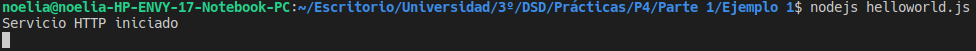
\includegraphics[totalheight=0.7cm]{img/1.png}
		\end{figure}
		\item Vamos a localhost:8080
		\begin{figure}[H]
			\centering
			
\includegraphics[totalheight=2cm]{img/2.png}
		\end{figure}
	\end{itemize}
	\section{Ejemplo 2}
	Se trata de una calculadora.
	\begin{itemize}
	\item Lanzamos el servicio
	\begin{figure}[H]
		\centering
		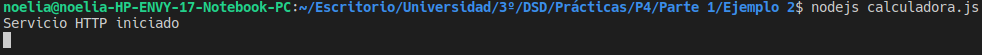
\includegraphics[totalheight=0.7cm]{img/3.png}
	\end{figure}
	\item Vamos a localhost:8080/sumar/2/3
	\begin{figure}[H]
		\centering
		
\includegraphics[totalheight=2cm]{img/4.png}
	\end{figure}
	\end{itemize}
	\section{Ejemplo 3}
	Tenemos una calculadora similar a la del ejemplo anterior pero con una interfaz.
	\begin{itemize}
		\item Lanzamos el servicio
		\begin{figure}[H]
			\centering
			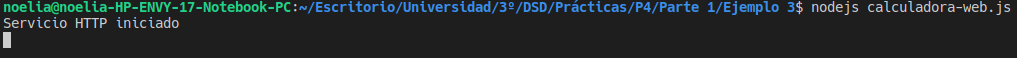
\includegraphics[totalheight=0.7cm]{img/5.png}
		\end{figure}
		\item Vamos a localhost:8080 e intentamos hacer una operación
		\begin{figure}[H]
			\centering
			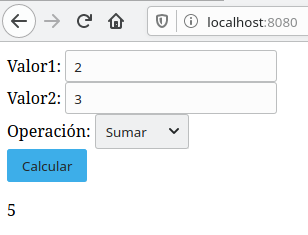
\includegraphics[totalheight=3cm]{img/6.png}
		\end{figure}
	\end{itemize}
	\section{Ejemplo 4}
	Se trata de un programa que muestra las conexiones activas actualmente.
	\begin{itemize}
		\item Lanzamos el servicio
		\begin{figure}[H]
			\centering
			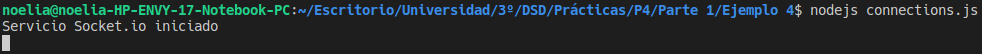
\includegraphics[totalheight=0.7cm]{img/7.png}
		\end{figure}
		\item Vamos a localhost:8080
		\begin{figure}[H]
			\centering
			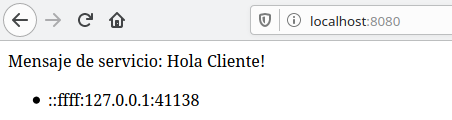
\includegraphics[totalheight=3cm]{img/8.png}
		\end{figure}
		\item En la terminal nos aparece el siguiente mensaje:
		\begin{figure}[H]
			\centering
			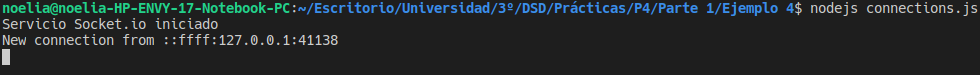
\includegraphics[totalheight=0.99cm]{img/9.png}
		\end{figure}
		\item Si abrimos otra pestaña de navegación
		\begin{figure}[H]
			\centering
			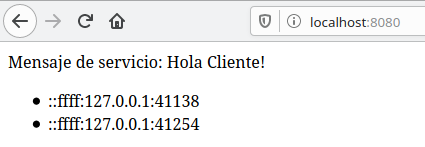
\includegraphics[totalheight=3cm]{img/10.png}
		\end{figure}
		\begin{figure}[H]
			\centering
			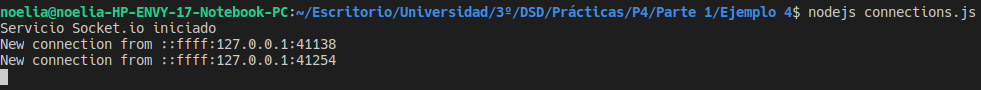
\includegraphics[totalheight=1.25cm]{img/11.png}
		\end{figure}
		\item Si ahora cerramos una ventana
		\begin{figure}[H]
			\centering
			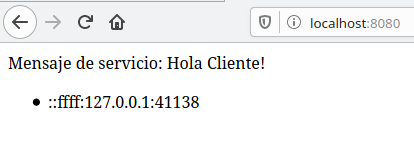
\includegraphics[totalheight=3cm]{img/12.png}
		\end{figure}
		\begin{figure}[H]
			\centering
			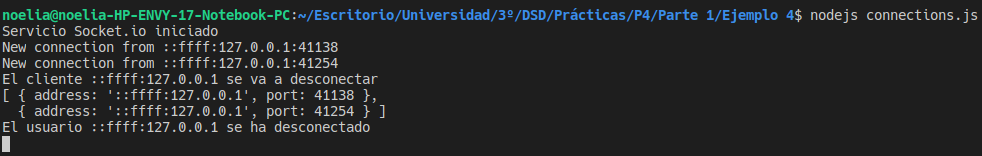
\includegraphics[totalheight=2.15cm]{img/13.png}
		\end{figure}
		\item Y si paramos el servicio
		\begin{figure}[H]
			\centering
			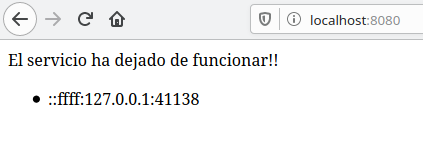
\includegraphics[totalheight=3cm]{img/14.png}
		\end{figure}
		\item Si lo volvemos a poner a funcionar se reconecta automáticamente.
		\begin{figure}[H]
			\centering
			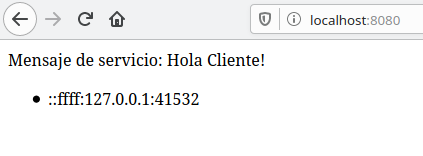
\includegraphics[totalheight=3cm]{img/15.png}
		\end{figure}
	\end{itemize}
	\section{Ejemplo 5}
	Se trata de un programa que guarda un histórico de conexiones.
	\begin{itemize}
		\item Lanzamos el servicio
		\begin{figure}[H]
			\centering
			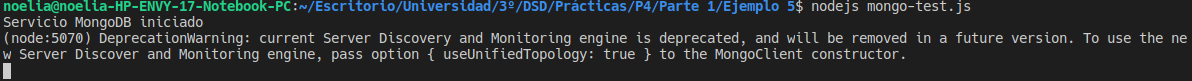
\includegraphics[totalheight=0.9cm]{img/16.png}
		\end{figure}
		\item Vamos a localhost:8080
		\begin{figure}[H]
			\centering
			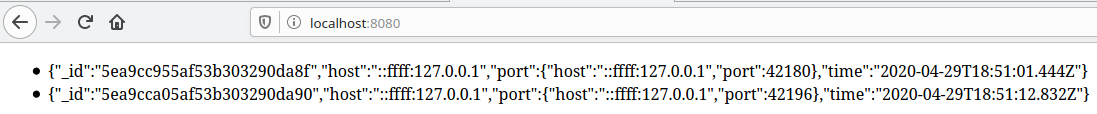
\includegraphics[totalheight=1.38cm]{img/17.png}
		\end{figure}
		\item Si abrimos otra pestaña se añadie otra conexión a la lista.
		\begin{figure}[H]
			\centering
			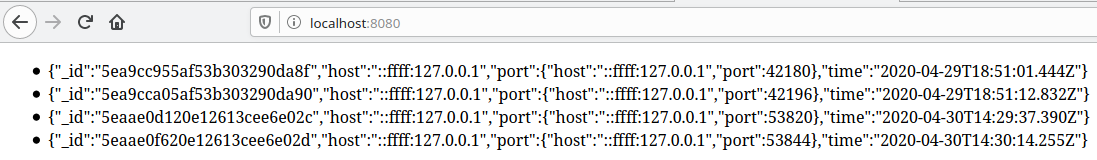
\includegraphics[totalheight=1.92cm]{img/18.png}
		\end{figure}
		Aunque detengamos el servicio y lo volvamos a iniciar se guardan las conexiones.
	\end{itemize}
\end{document}